\chapter{Methodologies}
\label{chap:methods}

This chapter illustrates the methodology used to approach the development process of this work.The application is divided into three main independent instances: gesture recognition, 3D trajectory detection and drone controller. First of all, the Section \ref{sec:handgestrec} to create a \gls{dnn} model to recognize hand gestures, followed by Section \ref{sec:getdata} and \ref{sec:model} that describes the type of data used for this purpose and how they are generated. After, we will see about how orientation and camera-hand distance has been estimated in Section \ref{sec:orientationestimation} and \ref{subsec:cam-hand} to detect a 3D trajectory. Next, we focus on the drone controller in simulation and real. We conclude Section \ref{sec:pipeline} with a detailed explanation of the entire pipeline.

%pipeline
%mediapipe (poco perché già parlato tecnicamente)
%costruzione della rete neurale:
%	come devono essere i dati
%trasformazione matriciale
%algoritmo dei tre punti orientamento
%pitch
%yaw
%roll

\section{Hand Gesture Recognition}
\label{sec:handgestrec}
MediaPipe has a python implementation for their Hand Keypoints Detector. It returns 2.5D coordinates of 21 hand landmarks (see Fig.\ref{fig:handland}), consisting of $x$, $y$, and relative $depth$. For this project the $depth$ coordinate of each hand landmark have been deleted because we wanted to estimate them.

% https://towardsdatascience.com/control-dji-tello-drone-with-hand-gestures-b76bd1d4644f

\begin{figure}[H]
	\centering
	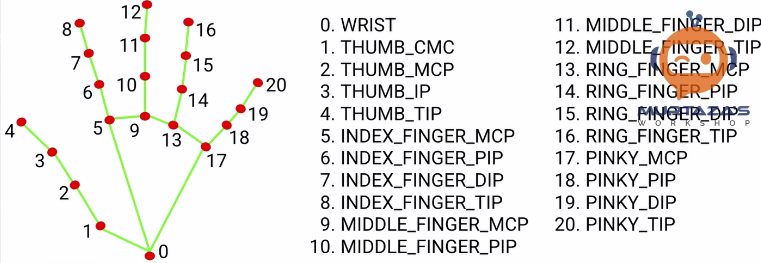
\includegraphics[width=.9\textwidth]{images/hand}
	\caption[Hand Landmarks.]{Image from the open MediaPipe repository.}
	\label{fig:handland}
\end{figure}

\noindent The coordinates of pixels in OpenCV follow a reference system $(x,y)$ in which the origin is in top-left of each image frame, $x$ is column-wise and $y$ is row-wise on the computer screen. In order to normalize each point, the origin was converted from top-left to bottom-left. This gave us the classic cartesian coordinate system. After, for each landmark was computed the mean for $x$ and $y$, converted in homogeneous coordinates and shifted them in order to match mean with origin. Note that shifting the data did not change how the data points are positioned relative to each other. Finally, each point has been scaled respect the max distance from mean point to all other hand points. This normalization permits to compare same gesture at different positions from the camera, if same orientation. 

\subsection{Data Acquisition and Description}
\label{sec:getdata}
Following the normalization of the data, it was thought of gestures that would allow firstly to acquire a 3D trajectory and secondly to interact directly with the drone. \\

\begin{figure}[H]
	\centering
	\includegraphics[width=1 \textwidth]{images/gestures}
	\caption[Full list of gestures.]{Full list of gestures that are available.}
	\label{fig:gestures}
\end{figure}

\noindent Below is the list of 10 gestures used in our project:
\begin{itemize}
	\item \texttt{backward}: this command allows the drone to go backwards;
	\item \texttt{detect}: this command allows you to detect a \gls{3d} trajectory;
	\item \texttt{down}: this command allows the drone to go down;
	\item \texttt{forward}: this command allows the drone to go forward;
	\item \texttt{land}: this command allows the drone to land;
	\item \texttt{left}: this command allows the drone to go left;
	\item \texttt{ok}: this command allows the drone to go close and execute a \gls{3d} trajectory;
	\item \texttt{right}: this command allows the drone to go right;
	\item \texttt{stop}: this command allows the drone to stop his movements;
	\item \texttt{up}: this command allows the drone to go up.
\end{itemize}

\noindent From the module that has been built is there the possibility to get data either from a webcam or from the drone camera. The dataset consists of $43$ columns: $42$ are the $21$ $2D$ points’ components, and the last is the target. $1000$ examples were acquired, $100$ images for each gesture. In total, the dataset is composed of $43000$ elements. The python script to get data has also a restore in case of particular error (for example if images are acquired from the drone could be problems due to overheating or low battery). Given the structure of the generation script it is particularly easy to build a model with new gestures.

\subsection{Pearson Correlation}
\label{sec:pearsoncorr}
Correlation is a measure of the linear relationship of 2 or more variables. Through correlation, we can predict one variable from the other. The logic behind using correlation for feature selection is that the good variables are highly correlated with the target. Furthermore, variables should be correlated with the target but should be uncorrelated among themselves.

\noindent If two variables are correlated, we can predict one from the other. Therefore, if two features are correlated, the model only really needs one of them, as the second one does not add additional information. We will use the Pearson Correlation here through the heatmap plot.

\noindent A heatmap is a two-dimensional graphical representation of data where the individual values that are contained in a matrix are represented as colors. The seaborn python package allows the creation of annotated heatmaps which can be tweaked using Matplotlib tools as per the creator’s requirement.

\begin{figure}[H]
	\makebox[\textwidth]{
		\includegraphics[width=1.3 \textwidth]{images/corr}
	}
	\caption[Heatmap.]{Heatmap is really useful to display a general view of numerical data, not to extract specific data point. It rapresents the correlation matrix and it is done using Pearson correlation.}\label{fig:correlation}
\end{figure}

% https://stats.stackexchange.com/questions/392517/how-can-one-interpret-a-heat-map-plot
% https://www.analyticsvidhya.com/blog/2020/10/feature-selection-techniques-in-machine-learning/
% https://towardsdatascience.com/feature-selection-with-pandas-e3690ad8504b
\noindent Each square shows the correlation between the variables on each axis. Correlation ranges from $-1$ to $+1$. Values closer to zero implies weaker correlation (exact $0$ implying no correlation). A value closer to $1$ implies stronger positive correlation, that is as one increases so does the other and the closer to $1$ the stronger this relationship is. A correlation closer to $-1$ is similar, but instead of both increasing, one variable will decrease as the other increases. This is called negative correlation.

\noindent The diagonals are all $1$ because those squares are correlating each variable to itself (so it's a perfect correlation). Larger the number associated (in absolute) the higher the correlation between the two variables. The plot is also symmetrical about the diagonal since the same two variables are being paired together in those squares. This is the reason why we we plot just the lower matrix.

\noindent Looking at the picture it is possible to see that there is a high correlation between variables. Therefore, we compared the correlation between features and remove one of two features that have an absolute correlation higher than $0.8$

\begin{figure}[H]
	\centering
	\includegraphics[width=1\textwidth]{images/featuresel}
	\caption[Feature Selection: Feature Vs Feature.]{Feature Selection: Feature Vs Feature.}
	\label{fig:featuresel}
\end{figure}

\noindent Note: a better verion could be used, setting an absolute value, saying $0.5$ as the threshold for selecting the variables. If we find that the predictor variables are correlated among themselves, we can drop the variable which has a lower correlation coefficient value with the target variable. High results are gained just finding that if the predictor variables are correlated among themselves we drop one of them. So we dropped all features except for $9$ features: WRIST\_X, WRIST\_Y, THUMB\_CMC\_X, INDEX\_FINGER\_MCP\_Y, INDEX\_FINGER\_PIP\_Y, MIDDLE\_FINGER\_MCP\_X, MIDDLE\_FINGER\_PIP\_X, MIDDLE\_FINGER\_DIP\_X, RING\_FINGER\_DIP\_Y. These are the final features given by Pearson correlation.

\subsection{PCA}
\label{sec:pca}
% https://www.reneshbedre.com/blog/principal-component-analysis.html#pca-interpretation
PCA is a classical multivariate (unsupervised machine learning) non-parametric dimensionality reduction method that used to interpret the variation in high-dimensional interrelated dataset (dataset with a large number of variables). PCA reduces the high-dimensional interrelated data to low-dimension by linearly transforming the old variable into a new set of uncorrelated variables called principal component (\gls{pc}) while retaining the most possible variation. The first component has the largest variance followed by the second component and so on. The first few components retain most of the variation, which is easy to visualize and summarise the feature of original high-dimensional datasets in low-dimensional space. PCA helps to assess which original samples are similar and different from each other.

\begin{figure}[htbp]
	\makebox[\textwidth]{
		\includegraphics[width=1.3 \textwidth]{images/bipca}
	}
	\caption[PCA - Biplot.]{After dimensionality reduction, there usually is not a particular meaning assigned to each principal component. The new components are just the two main dimensions of variation.}\label{fig:bipca}
\end{figure}

\noindent As PCA is based on the correlation of the variables, it usually requires a large sample size for the reliable output. The sample size can be given as the absolute numbers or as subjects to variable ratios. The minimum absolute sample size of $100$ or at least $10$ or $5$ times to the number of variables is recommended for PCA. On other hand, Comrey and Lee’s (1992) have a provided sample size scale and suggested the sample size of $300$ is good and over $1000$ is excellent.

\noindent As the number of \glspl{pc} is equal to the number of original variables, We should keep only the PCs which explain the most variance ($70-95\%$) to make the interpretation easier. More the PCs you include that explains most variation in the original data, better will be the PCA model. This is highly subjective and based on the user interpretation (Cangelosi et al., 2007).

\noindent For a lot of machine learning applications it helps to be able to visualize the dataset. Visualizing $2$ or $3$ dimensional data is not that challenging. However things are different when the dimension is above four. We can use PCA to reduce that n dimensional data into $2$ or $3$ dimensions so that we can plot and hopefully understand the data better. For this reason we can say that PCA can also be used for Data Visualization. 

\noindent PCA is effected by scale so we need to scale the features in our data before applying PCA. In sklearn framework using StandardScaler helps standardize the dataset’s features onto unit scale ($mean = 0$ and $variance = 1$) which is a requirement for the optimal performance of many machine learning algorithms. An alternative standardization is scaling features to lie between a given minimum and maximum value, often between zero and one, or so that the maximum absolute value of each feature is scaled to unit size. This can be achieved using MinMaxScaler or MaxAbsScaler, respectively. Problem about StandardScaler is when we have new data, and this cannot be scaled as the dataset used to build the \gls{ml} model. We have choosen MinMaxScaler. \\

\noindent Biplots (see Fig. \ref{fig:bipca}) are useful to visualize the relationships between variables and observations. The original data has $n$ columns and we projects the original data which is $m$ dimensional (where $m$ is the number of rows, in other words, the sample number of the dataset) into $2$ dimensions. From the biplot and loadings plot, we can see that a lot of variables are highly associated and forms cluster. If the variables are highly associated, the angle between the variable vectors should be as small as possible in the biplot. The length of PCs in biplot refers to the amount of variance contributed by the \glspl{pc}. The longer the length of \gls{pc}, the higher the variance contributed and well represented in space. The first two \glspl{pc} contribute $~70,43\%$ of the total variation in the dataset.

\noindent Scree plot (see Fig. \ref{fig:screeplot}) is another graphical technique useful in \glspl{pc} retention. We should keep the \glspl{pc} where there is a sharp change in the slope of the line connecting adjacent \glspl{pc}. We took just only the $6$ \gls{pc} because they descrive around the $93\%$ of the total variation in the dataset .

\begin{figure}[H]
	\centering
	\includegraphics[width=.8\textwidth]{images/screeplot}
	\caption[Scree plot.]{Scree plot.}
	\label{fig:screeplot}
\end{figure}

\subsection{Model}
\label{sec:model}
Now we are ready to choose a model. For classification tasks there are variety of different estimators/models that we can choose from. In the end, DNNClassifier from Tensorflow framework, with two hidden layers composed of $30$ and $10$ neurons each. Input layer is composed of $42$ elements and the output layer of 10 classes (see Fig. \ref{fig:handarch}). The model must choose among ten classes. The activation function is the Leaky ReLU and Adam the optimizer with learning rate $0.1$, decay steps $10000$ and decay rate $0.96$. About steps for the training phase has been chosen $3000$ as value. Loss is calculated by using softmax cross entropy.

% https://github.com/ashishpatel26/Tools-to-Design-or-Visualize-Architecture-of-Neural-Network
% http://alexlenail.me/NN-SVG/index.html

\begin{figure}[H]
	\makebox[\textwidth]{
		\includegraphics[width=1.1 \textwidth]{images/net}
	}
	\caption[Hand gesture reconognition \gls{nn}.] {\gls{dnn} image of the hand gesture recognition, generated by NNSVG\footnote{\url{http://alexlenail.me/NN-SVG/index.html}}. This is the specific case when all the $42$ variables were given as input.}
	\label{fig:handarch}
\end{figure}

\noindent Three models were genearated: one using the entire dataset, one using just only the selected features and finally one using PCA. Because of such a simple structure, high accuracy was reached for all of them. It is not required to retrain the model for each gesture in different illumination (or building a convolutional neural network), because MediaPipe takes over all the detection work.

\section{3D trajectory detection}
\label{sec:3dtraj}
Trajectories will be detected using the detect gesture (see Fig. \ref{fig:gestures} (c)). The experiments about orientation estimation will be executed just only on that gesture. 

\subsection{Orientation estimation}
\label{sec:orientationestimation}
% Note that yaw and pitch orientation estimates are made after the hand points are normalized, while roll is computed at the time of normalization, as described in. The normalization in this phase occurs by first of all making the translation so that the origin of the axes matches the midpoint of the hand, then all the points of the hand are scaled so that the maximum distance between them and the origin has a value of 1. Finally we rotate the hand with respect to the roll value computed during the normalization phase.
In the following section, we will discuss the methods used to perform yaw, roll and pitch measurements starting from the pixels of the image captured with a camera. Note that yaw and pitch orientation estimates are made after the hand points are normalized, while roll is computed at the time of normalization, as described in. The normalization in this phase occurs by first of all making the translation so that the origin of the axes matches the midpoint of the hand, then all the points of the hand are scaled so that the maximum distance between them and the origin has a value of 1. Finally we rotate the hand \gls{wrt} the roll value computed during the normalization phase.

\subsubsection{Turning and orientations}
\label{subsec:orientationtest}
%ATTENZIONE DA FARE (citare cmsc754-spring2020-lects)
In order to find a value for the yaw we need to understand how to determine whether three points form a left-hand turn. This can be done by an orientation test, which is fundamental to many algorithms in computational geometry (citare cmsc754-spring2020-lects). Given an ordered triple of points $\langle p, q, r \rangle$ in the plane, we say that they have positive orientation if they define a counterclockwise oriented triangle (see Fig. \ref{fig:orientationtest} (a)), negative orientation if they define a clockwise oriented triangle (see Fig. \ref{fig:orientationtest} (b)), and zero orientation if they are collinear, which includes as well the case where two or more of the points are identical (see Fig. \ref{fig:orientationtest} (c)). It is important take care about the fact that the orientation depends on the order in which the points are given.

\begin{figure}[H]
	\centering
	\includegraphics[width=.8\textwidth]{images/orientationtest}
	\caption[Orientation test.]{Orientations of the ordered triple (p, q, r).}
	\label{fig:orientationtest}
\end{figure}

\noindent Orientation is formally defined as the sign of the determinant of the points given in homogeneous coordinates, that is, by prepending a 1 to each coordinate. For example, in the plane, we define:

% https://jasonwarta.github.io/latex-matrix/ 
\begin{Equation}[!htb]
	\centering
	\begin{equation} \label{eq:orientationtest}
		Orient(p,q,r) = det
		\begin{pmatrix}
			1 & p_x & p_y \\
			1 & q_x & q_y \\
			1 & r_x & r_y 
		\end{pmatrix}
		\end{equation}
	\caption[Orientation test.]{Thus orientation generalizes the familiar 1-dimensional binary relations $<, =, >$.}
\end{Equation}

\noindent The sign of the orientation of an ordered triple is unchanged if the points are translated, rotated, or scaled (by a positive scale factor). In general, applying any affine transformation to the point alters the sign of the orientation according to the sign of the determinant of the matrix used in the transformation. \\

\noindent If we consider points belonging to the same reference system and compute the orientation test then we can get information of how much the points are crushed together. 

\subsubsection{Roll estimation}
\label{subsec:roll}
To estimate the roll, we found the angle generated by the vertical axis passing over the wrist and the tip of the middle finger (see fig. \ref{fig:handland}).

\subsubsection{Yaw estimation}
\label{subsec:yaw}
First of all, to estimate the yaw, it is necessary to fix a hand. This project will be on the left-hand, so each comment will be in that direction. Despite this, the same can be said for the right hand. Then, we compute the orientation test (see Eq. \ref{eq:orientationtest}) of three points $\langle p, q, r \rangle$. As already said, the order here is important to find the direction of orientation, therefore to know if the left-hand points left or right and with which intensity. We have seen empirically that if $roll < \ang{-5}$ or $roll > \ang{+5}$ it is better to consider $p=$ index\_finger\_mcp, $q=$ index\_finger\_pip and $r=$ index\_finger\_dip. Otherwise, if $\ang{-5} < roll < \ang{+5}$ we have noted that good results if $p=$ middle\_finger\_mcp, $q=$ middle\_finger\_pip and $r=$ middle\_finger\_dip. These hand points were chosen because they scale quite well with hand orientation. \\

\noindent The value of the orientation test is elevated to the second power, in order to be more stable around \ang{0}. Then, it is divided by $1666$, a value computed empirically to bring the results obtained from the orientation test to the range of \ang{-90} to \ang{+90}. Since we used the quadratic form, this value will be very huge if greater than \ang{+90} or smaller than \ang{-90}, for this reason the part the exceeds has been reduced to be just the $10\%$ of it.

\subsubsection{Pitch estimation}
\label{subsec:pitch}
To compute pitch estimation, we compute the middle point $m$ between index\_finger\_mcp and index\_finger\_pip and then the difference between $m$ and the thumb\_tip, respect vertical axis (see fig. \ref{fig:handland}). Also here, as for yaw estimation, the value obtained is elevated to the second power, in order to be more stable around \ang{0}. Then, we divided the result by $31$ (empirically computed), to bring the results to the range of \ang{-90} to \ang{90}. Since we used the quadratic form, also here if the value is greater than \ang{90} or smaller than \ang{-90} the results tends to be really big, therefore the part the exceeds has been reduced to be just the 10\% of it.

\subsection{Camera-hand distance estimation}
\label{subsec:cam-hand}
%Nella fase iniziale di identificazione di una traiettoria 3d, il palmo della mano è perpendicolare rispetto al raggio d'azione dalla lente della fotocamera. La mano all'inizio è ferma e nell'immagine acquisita la stessa mano possiede una certa area h. Se consideriamo il punto centrale p della mano come la distanza media tra tutti i punti di riferimento della mano allora tale punto p possiamo considerarlo l'origine di un sistema di riferimento cartesiano ortogonale a tre assi. 
%
%Se volessimo trattare la mano come un punto materiale, cioè che non cambia il suo orientamento nello spazio, allora catturare tutti i punti medi della mano e confrontare le aree della mano per stimare le profondità nel corso del tempo t significa ottenere quei punti che identificano una traiettoria 3d. 
%
%Se però volessimo trattare la mano come un corpo, e quindi stimare anche il suo orientamento nello spazio allora le cose si complicano. Infatti, seppur comunque riusciremmo a identificare lo spostamento bidimensionale della mano, in termini di altezza e larghezza, come se trattassimo la mano come un punto materiale, invece non potremmo più confrontare le aree della mano perché queste possono essere alterate a causa dell'orientamento della mano assunta in un certo istante di tempo. Ecco perchè abbiamo di stimare l'orientamento della mano nello spazio, perché così possiamo proiettare i punti che descrivono la mano in modo che la mano sia perpendicolare rispetto al raggio d'azione della lente della fotocamera, quindi a ricondurci al caso precedente, ovvero confrontare le aree della mano per stimare la profondità.

In the initial phase of identifying a 3D trajectory, the palm of the hand is perpendicular to the range of action from the camera lens. At the beginning the hand is still and in the acquired image the same hand has a certain area h. If we consider the central point p of the hand as the average distance between all the reference points of the hand then this point p can be considered the origin of an orthogonal three-axis Cartesian reference system.

\noindent If we wanted to treat the hand as a material point, i.e. that does not change its orientation in space, then capturing all the midpoints of the hand and comparing the areas of the hand to estimate the depths over time t means obtaining those points that identify a trajectory 3d.

\noindent However, if we wanted to treat the hand as a body, and therefore also estimate its orientation in space, then things get complicated. In fact, although we would still be able to identify the two-dimensional displacement of the hand, in terms of height and width, as if we were treating the hand as a material point, instead we could no longer compare the areas of the hand because these can be altered due to the orientation of the hand, taken in a certain instant of time. This is why we have to estimate the orientation of the hand in space, because in this way we can project the points that describe the first hand detected, thus bringing us back to the previous case, comparing areas of the hand to estimate depth. \\


%Quindi dopo aver rilevato il primo gesto, è stato calcolato il punto medio p e tutti punti della mano sono stati traslati in modo tale che il punto medio p diventi l'origine della mano. Notare che, a differenza di come è stato fatto per normalizzare i dati come ingresso per la rete neurale, qui non scaliamo i punti rispetto la massima distanza tra punto medio e tutti gli altri punti della mano. Non lo facciamo perché non vogliamo perdere l'informazione dello scaling. Anche tutti i gesti sucessivi (sempre riferiti al gesto del "detect") con possibile orientamento diverso vengono catturati ed eseguito lo stesso processo di normalizzazione. A ogni frame computiamo il valore della profondità confrontando la prima mano acqusita con quella in corso. Nello specifico, ai punti che definiscono la prima mano acquisita attuiamo una trasformazione matricale: una rotazione 3D lungo i 3 assi sfruttando le stime dello yaw, roll e pitch calcolare precedentmente

\noindent So after detecting the first gesture, the midpoint $p$ was calculated and all points of the hand were translated in such a way that the midpoint $p$ becomes the origin of the hand. Note that, unlike how it was done to normalize the data as an input to the neural network, here we do not scale the points \gls{wrt} the maximum distance between the midpoint and all other points of the hand. We do not do this because we do not want to lose the scaling information. Also all subsequent gestures (always referring to the "detect" gesture) with possible different orientation are captured and performed the same normalization process. At each frame we calculate the depth value by comparing the first hand acquired with the one in progress. Specifically, at the points that define the first hand acquired we implementd a matrix transformation: a 3D rotation along the 3 axes using the estimates of the yaw, roll and pitch calculated previously (see \ref{sec:orientationestimation}).

\noindent A rotation matrix rotates an object about one of the three coordinate axes or any arbitrary vector. The rotation matrix is more complex than the scaling and translation matrix since the whole $3x3$ upper-left matrix is needed to express complex rotations. It is common to specify arbitrary rotations with a sequence of simpler ones each along with one of the three cardinal axes. In each case, the rotation is through an angle, about the given axis. As in \ref{eq:rotx}, \ref{eq:roty} and \ref{eq:rotz}, the three matrices $R_X$, $R_Y$ and $R_Z$ represent transformations that rotate points through the angle $\theta$ in radians about the coordinate origin.

% FORSE MEGLIO INSERIRE LE ROATAZIONI CLASSICHE, MA PRIMA GUARDARE IL CODICE SE FUNZIONANO
\begin{Equation}[!htb]
	\centering
	\begin{equation} \label{eq:rotx}
	R_X(\theta) =
		\begin{pmatrix}
			1 & 0 & 0 & 0 \\
			0 & cos(\theta) & sin(\theta) & 0 \\
			0 & -sin(\theta) & cos(\theta) & 0 \\
			0 & 0 & 0 & 1 \\
		\end{pmatrix}
	\end{equation}
	\caption[X-Rotation Matrix in homogeneous coordinates.]{X-Rotation Matrix in homogeneous coordinates.}
\end{Equation}

\begin{Equation}[!htb]
	\centering
	\begin{equation} \label{eq:roty}
	R_Y(\theta) =
		\begin{pmatrix}
			cos(\theta) & 0 & -sin(\theta) & 0 \\
			0 & 1 & 0 & 0 \\
			sin(\theta) & 0 & cos(\theta) & 0 \\
			0 & 0 & 0 & 1 \\
		\end{pmatrix}
	\end{equation}
	\caption[Y-Rotation Matrix in homogeneous coordinates.]{Y-Rotation Matrix in homogeneous coordinates.}
\end{Equation}

\begin{Equation}[!htb]
	\centering
	\begin{equation} \label{eq:rotz}
	R_Z(\theta) =
		\begin{pmatrix}
			cos(\theta) & -sin(\theta) & 0 & 0 \\
			sin(\theta) & cos(\theta) & 0 & 0 \\
			0 & 0 & 1 & 0 \\
			0 & 0 & 0 & 1 \\
		\end{pmatrix}
	\end{equation}
	\caption[Z-Rotation Matrix in homogeneous coordinates.]{Z-Rotation Matrix in homogeneous coordinates.}
\end{Equation} 

\noindent It must be further defined whether positive angles perform a clockwise (CW) or counterclockwise (CCW) rotation around an axis \gls{wrt} a specification of the orientation of the axis. Here, positive rotation angles cause a counterclockwise rotation about an axis as one looks inward from a point on the positive axis toward the origin. This is commonly the case for right-handed coordinate systems. Note that transformation matrices containing only rotations and translations are examples of rigid-body (solid-body) transformations, which do not alter the size or shape of an object. It is also possible to combine the three transformations to obtain a single matrix (see Eq. \ref{eq:rot})

% SE CAMBI LE TRASFORMAZIONI PRECEDENTI ALLORA AGGIUNGI ANCHE IL FORUMULONE CHE è COMBINAZIONE DELLE 3
\begin{Equation}[H]
	\centering
	\begin{equation} \label{eq:rot}
		R(pitch, yaw, roll) = R_X(pitch) \cdot R_Y(yaw) \cdot R_Z(roll)
	\end{equation}
	\caption[General Rotation.]{General rotation matrix, used to perform a rotation in Euclidean space.}
\end{Equation}

\noindent Actually, instead of calculating the area of the hand, the mean of the sums of the distances between the hand midpoint p and all other reference hand landmark was calculated, to have a more robust metric. After having performed this last operation both on all the points of the current hand and on the first hand transformed with the general matrix, we finally made the difference between the first and the second value obtained previously. In this way we are able to obtain an estimate of the depth of the hand (which is performing the detecting gesture) even if it is oriented in space.

\subsection{Univariate spline}
\label{sec:univspline}
Fitting data

\section{Drone controller}
\label{sec:dronecontrl}

\subsection{Simulation}
\label{sec:simulation}

\subsection{Real world}
\label{sec:simulation}

\section{Pipeline}
\label{sec:pipeline}
